% Copyright (c) 2021 Eclipse Arrowhead Project
%
% This program and the accompanying materials are made available under the
% terms of the Eclipse Public License 2.0 which is available at
% http://www.eclipse.org/legal/epl-2.0.
%
% SPDX-License-Identifier: EPL-2.0

This section is what constitutes the \GlossaryHyperRef{model-reference}{reference model} of this document.
Each of its subsections \GlossaryHyperRef{description}{describes} a primary Arrowhead concept, which are as follows:

\vspace*{0.5cm}

\noindent\begin{tabularx}{\textwidth}{@{} p{0.9cm} p{4.3cm} X @{}}

\ref{sec:reference-model:stakeholder}                              & \textbf{\nameref{sec:reference-model:stakeholder}}                              & A person or \GlossaryHyperRef{organization}{organization} with \GlossaryHyperRef{stake}{stake} in an \GlossaryHyperRef{entity}{entity} or undertaking. \\
\ref{sec:reference-model:entity}                                   & \textbf{\nameref{sec:reference-model:entity}}                                   & An \GlossaryHyperRef{artifact}{artifact} that can be distinguished from all other artifacts. \\
\ref{sec:reference-model:device}                                   & \textbf{\nameref{sec:reference-model:device}}                                   & A physical \GlossaryHyperRef{entity}{entity} with the significant \GlossaryHyperRef{capability}{capability} of being able to host \GlossaryHyperRef{system}{systems}. \\
\ref{sec:reference-model:system}                                   & \textbf{\nameref{sec:reference-model:system}}                                   & A \GlossaryHyperRef{instance-software}{software instance} able to exercise the \GlossaryHyperRef{capability}{capabilities} of its hosting \GlossaryHyperRef{device}{device}. \\
\ref{sec:reference-model:service}                                  & \textbf{\nameref{sec:reference-model:service}}                                  & A set of \GlossaryHyperRef{function}{functions} \GlossaryHyperRef{provider-service}{provided} by a \GlossaryHyperRef{system}{system} for other systems to \GlossaryHyperRef{consumer-service}{consume}. \\
\ref{sec:reference-model:system-of-systems}                        & \textbf{\nameref{sec:reference-model:system-of-systems}}                        & A set of \GlossaryHyperRef{system}{systems} together facilitating new \GlossaryHyperRef{capability-system}{capabilities}. \\
\ref{sec:reference-model:system-of-systems:local-cloud}            & \textbf{\nameref{sec:reference-model:system-of-systems:local-cloud}}            & A \GlossaryHyperRef{cloud}{cloud} with a \GlossaryHyperRef{boundary-local}{local boundary} and \GlossaryHyperRef{resource-local}{local resources}.\\
\ref{sec:reference-model:system-of-systems:system-of-local-clouds} & \textbf{\nameref{sec:reference-model:system-of-systems:system-of-local-clouds}} & A set of \GlossaryHyperRef{cloud-local}{local clouds} that jointly facilitate new \GlossaryHyperRef{capability-system}{capabilities}.\\
\ref{sec:reference-model:network}                                  & \textbf{\nameref{sec:reference-model:network}}                                  & A set of \GlossaryHyperRef{device}{devices} whose \GlossaryHyperRef{system}{systems} can \GlossaryHyperRef{communication}{communicate}.\\
\ref{sec:reference-model:interface}                                & \textbf{\nameref{sec:reference-model:interface}}                                  & A \GlossaryHyperRef{boundary}{boundary} that can be crossed by \GlossaryHyperRef{message}{messages} of certain \GlossaryHyperRef{protocol}{protocols}.\\
\ref{sec:reference-model:policy}                                   & \textbf{\nameref{sec:reference-model:policy}}                                   & A set of \GlossaryHyperRef{constraint}{constraints} that must be satisfied for an activity to be permitted.\\
\ref{sec:reference-model:protocol}                                 & \textbf{\nameref{sec:reference-model:protocol}}                                 & A \GlossaryHyperRef{description}{description} of how \GlossaryHyperRef{message}{messages} may be sent between \GlossaryHyperRef{entity}{entities}.\\

\end{tabularx}

\subsection{Stakeholder}
\label{sec:reference-model:stakeholder}

A \GlossaryHyperRef{stakeholder}{stakeholder} is a person or \GlossaryHyperRef{organization}{organization} with \GlossaryHyperRef{stake}{stake} in an \GlossaryHyperRef{entity}{entity} or undertaking with relevance to the \GlossaryHyperRef{framework-arrowhead}{Arrowhead framework}.
In this context, we understand \textit{stake} to refer to any type of engagement or commitment.
The concept is illustrated in Figure \ref{fig:stakeholder}, which also lists five reasons why a given person or organization could be considered to be a stakeholder.
We refer to these reasons as \GlossaryHyperRef{role-stakeholder}{\textit{roles}}.

\vspace*{0.3cm}

\begin{figure}[ht!]
  \centering
  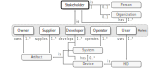
\includegraphics[scale=0.9]{figures/stakeholder}
  \caption{
    The stakeholder as either a person or organization, where each such stakeholder takes on one ore more distinct roles.
    The depicted roles is not an exhaustive list.
    \GlossaryHyperRef{hid}{HID} is an abbreviation for \GlossaryHyperRef{device-human-interface}{Human Interface Device}.
  }
  \label{fig:stakeholder}
\end{figure}

\vspace*{0.1cm}

The roles occupied by a given stakeholder dictates what \GlossaryHyperRef{entity}{entities} that person or organization will interact with, as well as the nature of that interaction.
In Figure \ref{fig:stakeholder}, (1) \GlossaryHyperRef{owner}{owner}, (2) \GlossaryHyperRef{designer}{designer}, (3) \GlossaryHyperRef{developer}{developer}, (4) \GlossaryHyperRef{operator}{operator} and (5) \GlossaryHyperRef{user}{user} are named explicitly, but more roles are likely to be relevant, such as (6) \GlossaryHyperRef{integrator}{integrator} and (7) \GlossaryHyperRef{engineer-standardization}{standardization engineer}, (8) \GlossaryHyperRef{researcher}{researcher}, and (9) \GlossaryHyperRef{manager}{manager}.
The listed nine names should be used rather than any synonyms when referring to these particular roles.
Please refer to the \hyperref[sec:glossary]{glossary} for their definitions.

\subsection{Entity}
\label{sec:reference-model:entity}

An \GlossaryHyperRef{entity}{entity} is an \GlossaryHyperRef{artifact}{artifact} that can be distinguished from all other artifacts.
We use the word \textit{artifact} to refer to any object or thing, physical or intangible.
As depicted in Figure \ref{fig:entity}, this means that an entity always has an \GlossaryHyperRef{identity}{identity}.

\begin{figure}[ht!]
  \centering
  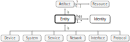
\includegraphics[scale=0.9]{figures/entity}
  \caption{
    The entity as an artifact with an identity.
    An entity or artifact may or may not be considered to be a \GlossaryHyperRef{resource}{resource}, in which case it is deemed to be of value to a \GlossaryHyperRef{stakeholder}{stakeholder}.
    The group of entity types is not exhaustive.
    Other examples are \GlossaryHyperRef{cloud-local}{local clouds}, certain \GlossaryHyperRef{data}{data}, \GlossaryHyperRef{policy}{policies}, \GlossaryHyperRef{protocol}{protocols} and \GlossaryHyperRef{profile}{profiles}.
  }
  \label{fig:entity}
\end{figure}

\vspace*{0.9mm}

Note that having an identity is not the same as being associated with an \GlossaryHyperRef{identifier}{identifier}, which is a name, number or other value referring to the entity in question.
It is enough that such an identifier could be produced for an artifact to count as an entity.
That being said, certain \GlossaryHyperRef{identification}{identification} requirements, perhaps related to security, performance or discoverability, may make it practically unfeasible not to use identifiers.

\subsection{Device}
\label{sec:reference-model:device}

A \GlossaryHyperRef{device}{device} is a physical \GlossaryHyperRef{entity}{entity} with the significant \GlossaryHyperRef{capability}{capability} of being able to host at least one \GlossaryHyperRef{system}{system}, each of which may be given the opportunity to exercise the capabilities of that device.
Examples of capabilities include moving robotic arms, reading from sensors, running \GlossaryHyperRef{procedure-software}{software procedures}, and sending \GlossaryHyperRef{message}{messages}. 
Every device consists of \GlossaryHyperRef{component-hardware}{hardware components}.
While there are no limits to what components can make up a device, each device must always have (1) \GlossaryHyperRef{unit-memory}{memory}, (2) \GlossaryHyperRef{unit-compute}{compute} and (3) \GlossaryHyperRef{interface-device}{interfacing} components, as shown in Figure \ref{fig:device}.

\begin{figure}[ht!]
  \centering
  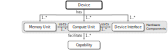
\includegraphics[scale=0.9]{figures/device}
  \caption{
    The device as an entity with hardware components, together facilitating one or more capabilities.
    Devices must be able to host systems, even if not made explicit by this figure.
    The group of hardware components is not exhaustive.
    Other examples of such components could be sensors, actuators, compute accelerators, or batteries.
  }
  \label{fig:device}
\end{figure}

\vspace*{1.8mm}

Devices must be able to host systems, or they must be considered as hardware components.
While it may seem unintuitive to consider certain machines as components, such as large pumping complexes or vehicles with only manual controls, the \GlossaryHyperRef{framework-arrowhead}{Arrowhead framework} is meant to facilitate automation through the use of interconnected devices with compute capabilities.
If a machine cannot run \GlossaryHyperRef{software}{software}, making it able to host systems, that capability must be added before it can play a meaningful role in an Arrowhead context.
Consequently, machines without system hosting capabilities must either be considered as components or not be considered from the perspective of Arrowhead at all.

\subsection{System}
\label{sec:reference-model:system}

A \GlossaryHyperRef{system}{system} is an \GlossaryHyperRef{identification}{identifiable} \GlossaryHyperRef{instance-software}{software instance} that is able to exercise the \GlossaryHyperRef{capability}{capabilities} of its hosting \GlossaryHyperRef{device}{device}.
As shown in Figure \ref{fig:system}, systems consists of \GlossaryHyperRef{component-software}{software components}.
Some significant such components are (1) \GlossaryHyperRef{state-software}{states}, (2) \GlossaryHyperRef{procedure-software}{procedures} and (3) \GlossaryHyperRef{interface-system}{system interfaces}, which are facilitated by the (1) \GlossaryHyperRef{unit-memory}{memory}, (2) \GlossaryHyperRef{unit-compute}{compute} and (3) \GlossaryHyperRef{interface-device}{interfacing} components of a device.
A system with these components should be able to \GlossaryHyperRef{consumer-service}{consume} and/or \GlossaryHyperRef{provider-service}{provide} \GlossaryHyperRef{service}{services}, or it must be referred to as an \GlossaryHyperRef{system-isolated}{\textit{isolated system}}.

\begin{figure}[ht!]
  \centering
  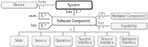
\includegraphics[scale=0.9]{figures/system}
  \caption{
    The system as a collection of related software components, able to trigger zero or more capabilities of its hosting device.
    The group of software components is not exhaustive.
    Other examples of such components could be operating systems, file systems, software libraries, programming language runtimes, databases or virtual machines.
  }
  \label{fig:system}
\end{figure}

This rather open-ended definition of ``system'' makes it possible for such to be realized in many ways.
A system may or may not run in its own operating system process, use a certain virtual machine, and so on.

\subsection{Service}
\label{sec:reference-model:service}

A \GlossaryHyperRef{service}{service} is an \GlossaryHyperRef{identification}{identifiable} set of \GlossaryHyperRef{function-service}{functions} \GlossaryHyperRef{provider-service}{provided} by a \GlossaryHyperRef{system}{system}, allowing for other systems to trigger its \GlossaryHyperRef{capability-system}{capabilities} by sending \GlossaryHyperRef{message}{messages} to, or \GlossaryHyperRef{invocation-function}{\textit{invoking}}, those functions.
The act of sending a message to a certain function is referred to as \GlossaryHyperRef{consumer-service}{\textit{consuming}} its service.
As depicted in Figure \ref{fig:service}, every service consists of at least three \GlossaryHyperRef{component-software}{software components}.
These are (1) \GlossaryHyperRef{state-software}{states}, (2) \GlossaryHyperRef{function-service}{functions} and (3) \GlossaryHyperRef{interface-service}{service interfaces}.

\begin{figure}[ht!]
  \centering
  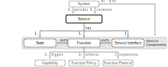
\includegraphics[scale=0.9]{figures/service}
  \caption{
    The service as means for a consuming system to trigger capabilities of a providing system.
    The group of software components is not exhaustive.
    See the caption of Figure \ref{fig:system} for additional examples.
  }
  \label{fig:service}
\end{figure}

Services receive messages via their interfaces, which must \GlossaryHyperRef{routing-message}{route} them to the functions they target.
A function receiving a message must guarantee that it adheres to its \GlossaryHyperRef{protocol-function}{protocol} and satisfies all of its \GlossaryHyperRef{policy-function}{policies}, after which it must concretely handle the request described in the message.
The function protocol dictates what \GlossaryHyperRef{data}{data} must be in the message, among other things, while the function policies may require that certain authorization tokens can be presented, that a future time slot in a real-time network has been allocated, and so on.

If it becomes relevant to distinguish the functions of programming languages with those introduced here, they should be referred to as \GlossaryHyperRef{function-program}{\textit{program functions}} and \GlossaryHyperRef{function-service}{\textit{service functions}}, respectively.
Otherwise the unqualified use of the word \textit{function} must be understood to refer to service functions.

\subsection{System-of-Systems}
\label{sec:reference-model:system-of-systems}

A \GlossaryHyperRef{system-of-systems}{system-of-systems} is an \GlossaryHyperRef{identification}{identifiable} set of at least two \GlossaryHyperRef{system}{systems}, together facilitating one or more \GlossaryHyperRef{capability-system}{capabilities} none of the constituent systems could have on its own.
While this definition may initially seem rather strict, it is enough for a system to \GlossaryHyperRef{consumer-service}{consume} a \GlossaryHyperRef{service}{service} of another system for a system-of-systems to emerge.
This as service consumption can only be motivated by the desire to facilitate new capabilities.

As illustrated in Figure \ref{fig:system-of-systems}, there are two types of systems-of-systems of particular relevance to the \GlossaryHyperRef{framework-arrowhead}{Arrowhead framework}, (1) the \GlossaryHyperRef{cloud-local}{local cloud} and (2) the \GlossaryHyperRef{system-of-local-clouds}{system-of-local-clouds}, which we describe in the following sections.

\begin{figure}[ht!]
  \centering
  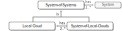
\includegraphics[scale=0.9]{figures/system-of-systems}
  \caption{
    The system-of-system as a group of two or more systems, together facilitating new capabilities.
  }
  \label{fig:system-of-systems}
  \vspace*{-3mm}
\end{figure}

\subsubsection{Local Cloud}
\label{sec:reference-model:system-of-systems:local-cloud}

A \GlossaryHyperRef{cloud-local}{local cloud} is a \GlossaryHyperRef{system-of-systems}{system-of-systems} able to execute given tasks through the use of a pool of \GlossaryHyperRef{resource}{resources}.
As depicted in Figure \ref{fig:local-cloud}, the local cloud is distinct from other types of \GlossaryHyperRef{cloud}{clouds} by having at least one \GlossaryHyperRef{boundary-local}{local boundary} and one \GlossaryHyperRef{resource-local}{local resource}, which means that it is physically tied to a concrete location.
A local cloud could be engaged in manufacturing, repairs, heating, electricity distribution, workspace monitoring, drone fleet control, among many other possible kinds of physical activities.
A local cloud may be stationary or mobile.
A cloud that has no resources or boundaries tied to any particular physical locations should be referred to as a \GlossaryHyperRef{cloud-virtual}{\textit{virtual cloud}}.

\begin{figure}[ht!]
  \centering
  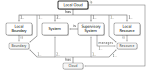
\includegraphics[scale=0.9]{figures/local-cloud}
  \caption{
    The local cloud as a regular cloud with at least one local boundary and one local resource.
  }
  \label{fig:local-cloud}
\end{figure}

That a local cloud has a boundary means that a distinction is being made between \GlossaryHyperRef{system}{systems} inside and outside the cloud.
A boundary being local means that the distinction is being made by a physical \GlossaryHyperRef{property}{property}, such as device location, type of device, or physical attachment to a certain \GlossaryHyperRef{entity}{entity}.
Boundaries may be protected, which means that measures are in place to guarantee security, safety, real-time characteristics, or other local cloud properties.
The resources of a local cloud may be of any type, from virtual compute resources to physical drills or pumps.
A system managing a resource may be referred to as a \GlossaryHyperRef{system-supervisory}{\textit{supervisory system}}.

\subsubsection{System-of-Local-Clouds}
\label{sec:reference-model:system-of-systems:system-of-local-clouds}

A \GlossaryHyperRef{system-of-local-clouds}{system-of-local-clouds} is two or more \GlossaryHyperRef{cloud-local}{local clouds} that \GlossaryHyperRef{consumer-service}{consume} each other's \GlossaryHyperRef{service}{services} to facilitate new \GlossaryHyperRef{capability-system}{capabilities}.
It is similar to the local cloud, with the exception of its \GlossaryHyperRef{subsystem}{subsystems} are \GlossaryHyperRef{cloud-local}{local clouds} instead of plain \GlossaryHyperRef{system}{systems}.
It has at least one common \GlossaryHyperRef{boundary-cloud}{boundary}, but no resources beyond those of its constituent clouds.

\subsection{Network}
\label{sec:reference-model:network}

A \GlossaryHyperRef{network}{network} is a set of two or more \GlossaryHyperRef{device-end}{end devices}, \GlossaryHyperRef{connection}{connected} in such a manner that any \GlossaryHyperRef{system}{systems} they host are able to \GlossaryHyperRef{communication}{communicate}.
As shown in Figure \ref{fig:network}, end devices may be \GlossaryHyperRef{interconnection}{interconnected} via \GlossaryHyperRef{device-intermediary}{intermediary devices}.

\begin{figure}[ht!]
  \centering
  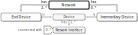
\includegraphics[scale=0.9]{figures/network}
  \caption{
    The network as a set of connected end devices, potentially interconnected by intermediary devices.
  }
  \label{fig:network}
\end{figure}

Both end devices and intermediary devices are regular \GlossaryHyperRef{device}{devices}, which means that they have \GlossaryHyperRef{interface-device}{device interfaces} through which they can send and receive \GlossaryHyperRef{message}{messages}.
Only \GlossaryHyperRef{device-connected}{\textit{connected} devices} can pass messages between their interfaces, however.
Intermediary devices pass on messages toward their intended end devices instead of handling them themselves.
Examples of intermediary devices are routers, switches, and firewalls.
Device interfaces used exclusively for passing on messages are referred to as \GlossaryHyperRef{interface-network}{network interfaces}.
Use of the term ``end device'' is only recommended when a distinction needs to be made between end and intermediary devices.

\subsection{Interface}
\label{sec:reference-model:interface}

An \GlossaryHyperRef{interface}{interface} is a \GlossaryHyperRef{boundary}{boundary} where \GlossaryHyperRef{message}{messages} of certain \GlossaryHyperRef{protocol}{protocols} can pass between a \GlossaryHyperRef{connection}{connection} and an \GlossaryHyperRef{entity}{entity}, between two entities, or between an entity and a person.
As outlined in Figure \ref{fig:interface}, there are three types of interfaces of particular relevance, (1) the \GlossaryHyperRef{interface-device}{device interface}, (2) the \GlossaryHyperRef{interface-system}{system interface}, and (3) the \GlossaryHyperRef{interface-service}{service interface}.

\begin{figure}[ht!]
  \centering
  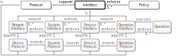
\includegraphics[scale=0.9]{figures/interface}
  \caption{
    The interface as the boundary where messages pass between mediums and entities.
  }
  \label{fig:interface}
\end{figure}

Device interfaces connect \GlossaryHyperRef{device}{devices}, system interfaces connect \GlossaryHyperRef{system}{systems}, and service interfaces connect \GlossaryHyperRef{consumer-service}{service consumers} with \GlossaryHyperRef{provider-service}{service providers}.
Each of these interface levels depend on the layer below it, with the exception of the device interface at the bottom.
As each interface supports its own set of protocols, each interface layer must support a protocol that extends that of the below layer.
A device interface may, for example, support the IP \cite{deering2017internet} protocol via Ethernet \cite{iso202188023}, a system interface the HTTP \cite{fielding2014hypertext} protocol via TCP \cite{postel1981transmission}, and a service interface a custom HTTP extension enabling it to \GlossaryHyperRef{router-message}{route} messages to the \GlossaryHyperRef{function-service}{functions} of its \GlossaryHyperRef{service}{service}.
Note that the protocol at each layers may consist of multiple protocols extending each other, as in this example.
A particular chain of protocols supported by a device, system or service is referred to as a \GlossaryHyperRef{stack-protocol}{\textit{protocol stack}}.
The protocol stack of the system in the previous example would be Ethernet, IP, TCP and HTTP, from the bottom and up.

\newpage

\subsection{Policy}
\label{sec:reference-model:policy}

A \GlossaryHyperRef{policy}{policy} is a set of \GlossaryHyperRef{constraint}{constraints}, of any nature, that must be satisfied for a certain activity to be permitted.
Policies may be concerned with authorization, contracts, economic goals, and so on.
As depicted in Figure \ref{fig:policy}, there are two categories of policies of particular relevance, (1) \GlossaryHyperRef{policy-service}{service policies} and (2) \GlossaryHyperRef{policy-function}{function policies}.

\begin{figure}[ht!]
  \centering
  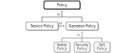
\includegraphics[scale=0.9]{figures/policy}
  \caption{
    The two categories of policies of highest relevance to this reference model, service and function policies, as well as some examples of possible function policies.
    \GlossaryHyperRef{qos}{QoS} is an abbreviation for \GlossaryHyperRef{service-quality-of}{quality of service}.
    The group of policy types is not exhaustive.
    Other examples could be real-time, pollution or certificate policies.
  }
  \label{fig:policy}
\end{figure}

A function policy must be satisfied for a system to be allowed to \GlossaryHyperRef{consumer-service}{consume} a particular \GlossaryHyperRef{function-service}{service function}.
A service policy, or a \textit{service-level} policy, applies to all \GlossaryHyperRef{function-service}{functions} of a given \GlossaryHyperRef{service}{service}.
Failing to satisfy a policy should mean that the consumer in question is notified about the specific policy or policies being violated.

\subsection{Protocol}
\label{sec:reference-model:protocol}

A \GlossaryHyperRef{protocol}{protocol} is a \GlossaryHyperRef{description}{description} of how certain \GlossaryHyperRef{message}{messages} may be sent between \GlossaryHyperRef{entity}{entities} as dictated by zero or more \GlossaryHyperRef{state-protocol}{states}.
Received messages may be rejected by violating a current state, or cause a state to be updated.
States may also be updated by other events. 
As illustrated in Figure \ref{fig:protocol}, a protocol may be defined as an \GlossaryHyperRef{protocol-extensible}{extension} of another protocol, may be constrained by \GlossaryHyperRef{profile-protocol}{profiles}, and defines its messages in terms of at least one \GlossaryHyperRef{encoding}{encoding}.

\begin{figure}[ht!]
  \centering
  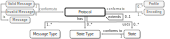
\includegraphics[scale=0.9]{figures/protocol}
  \caption{
    The protocol as set of state and message types, constrained by profiles and encodings.
  }
  \label{fig:protocol}
\end{figure}

A profile narrows down what a particular protocol is permitted to express, for example by requiring that authorization tokens be included in requests, or that a certain message payload semantics be observed.
Adding a profile to a protocol not already conforming to it produces a new protocol.
An encoding introduces a \GlossaryHyperRef{system-type}{type system} in which message payloads can be expressed.
If a protocol defines its messages without referring to an encoding, it is considered to have a \textit{custom} encoding.
